\normalfalse \difficiletrue \tdifficilefalse
\correctionfalse

%\UPSTIidClasse{11} % 11 sup, 12 spé
%\newcommand{\UPSTIidClasse}{12}

\exer{Circuit électrique$\star$ \label{C1:06:536}}

\setcounter{numques}{0}
\UPSTIcompetence[2]{C1-06}
\index{Compétence C1-06}
\index{Grandeurs électriques}
\index{Lois de Kirchhoff}
\ifcorrection
\else
\textbf{Pas de corrigé pour cet exercice.}
\fi

\question{Sur le circuit suivant, déterminer les courants dans chacune des branches et la tension aux bornes de tous les dipôles en fonction de $E$ et des différentes résistances $R_i$.}

\ifprof
\else

\begin{center}
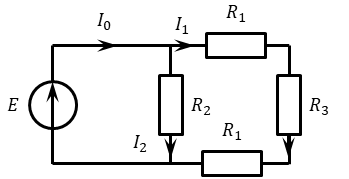
\includegraphics[width=\linewidth]{536_01}
\end{center}

\fi



\ifprof
\else
\begin{flushright}
\footnotesize{Corrigé  voir \ref{C1:06:536}.}
\end{flushright}%
\fi